\documentclass[beamer, en, version=2.0]{huangfusl-template}
\usepackage[scheme=plain]{ctex}
\usepackage{listings}
\usepackage{libertine}
\usefonttheme[onlymath]{serif}
% Change tt font to Source Code Pro
\usepackage{sourcecodepro}
\lstset{
    basicstyle=\ttfamily\footnotesize,
    backgroundcolor=\color{darkblue!10},
    % Set color paddings
    frame=single,
    framerule=0pt,
    breakatwhitespace=true,
    showstringspaces=false,
    % Set comment to gray and italic
    commentstyle=\color{gray}\itshape,
    % Set keyword to bold and darkblue
    keywordstyle=\color{darkblue}\bfseries,
    % Set string to darkred
    stringstyle=\color{darkred},
}

\title[Lecture 2: Advanced Python Programming]{\LARGE{清华经管博士生工作坊}\newline\newline \large{Lecture 2: Advanced Python Programming}}
\author{皇甫硕龙}
\date{2024-04-25}
\splitsections

\begin{document}
    \begin{frame}[fragile]
        \maketitle
    \end{frame}
    \section{Review of Last Lecture}
    \begin{frame}
        \frametitle{Review of Last Lecture}

        In the last lecture, we have covered the following topics:

        \begin{enumerate}
            \item Expressions and assignments
            \item Python basic data types and data structures
            \item Operators
            \item Control flow structures
            \item Defining and calling functions
        \end{enumerate}
    \end{frame}
    \begin{frame}[fragile]
        \frametitle{Examples}

        \begin{block}{Example 1: Size of rectangle}
            Read the length and width of a rectangle from the user, and calculate the area of the rectangle.
        \end{block}

        Key points: variable assignment, type conversion, input/output, arithmetic operations, f-strings.

        \pause

\begin{lstlisting}[language=python]
length = float(input('Enter the length: '))
width = float(input('Enter the width: '))
area = length * width
print(f'The area of the rectangle is {area}.')
\end{lstlisting}
    \end{frame}
    \begin{frame}[fragile]
        \frametitle{Examples}

        \begin{block}{Example 2: Factorial}
            Read a positive integer $n$ from the user, and calculate the factorial of $n$.
        \end{block}

        Key points: loops.

        \pause

\begin{lstlisting}[language=python]
n = int(input('Enter a positive integer: '))
factorial = 1
for i in range(1, n + 1):
    factorial *= i
print(f'The factorial of {n} is {factorial}.')
\end{lstlisting}

    \end{frame}
    \begin{frame}[fragile]
        \frametitle{Example}

        \begin{block}{Example 3: Determine whether a year is a leap year}
            Read a year from the user, and determine whether it is a leap year.
        \end{block}

        Key points: conditional statements.

        \pause

\begin{lstlisting}[language=python]
year = int(input('Enter a year: '))
if (year % 4 == 0 and year % 100 != 0) or year % 400 == 0:
    print(f'{year} is a leap year.')
else:
    print(f'{year} is not a leap year.')
\end{lstlisting}
    \end{frame}
    \begin{frame}[fragile]
        \frametitle{Example}

        \begin{block}{Example 4: Fibonacci sequence}
            Read a positive integer $n$ from the user, and print leading $n$ numbers in the Fibonacci sequence. The first two numbers in the sequence are 0 and 1, and each subsequent number is the sum of the two preceding numbers.
        \end{block}

        Key points: loops, variables, list operations, list reverse indexing.

        \pause

\begin{lstlisting}[language=python]
def fibonacci(n):
    fib = [0, 1]
    while len(fib) < n:
        fib.append(fib[-1] + fib[-2])
    return fib
n = int(input('Enter a positive integer: '))
print(fibonacci(n))
\end{lstlisting}
    \end{frame}
    \begin{frame}[fragile]
        \frametitle{Example}

        \begin{block}{Example 5: Split a string}
            Read a string from the user, and split it into words. Print the words in reverse order.
        \end{block}

        Key points: string operations, list operations.

        \pause

\begin{lstlisting}[language=python]
sentence = input('Enter a sentence: ')
words = sentence.split()
print(' '.join(words[::-1]))
\end{lstlisting}
    \end{frame}
    \begin{frame}[fragile]
        \frametitle{Example}

        \begin{block}{Example 6: Count the frequency of words}
            Read a string from the user, and count the frequency of each word in the string.
        \end{block}

        Key points: loop, string operations, dictionary operations.

        \pause

\begin{lstlisting}[language=python]
sentence = input('Enter a sentence: ')
words = sentence.split()
word_freq = {}

for word in words:
    word_freq[word] = word_freq.get(word, 0) + 1
print(word_freq)
\end{lstlisting}

    \end{frame}
    \section{Annotation and Type Checking}
    \begin{frame}
        \frametitle{Why Annotation}

        \only<1>{
        IDE and other text editors can provide auto completions. Annotations can help the editor to provide better auto completions.

        \begin{columns}
        \begin{column}{0.5\textwidth}
            \begin{block}{Without annotation}
                \begin{figure}[h]
                    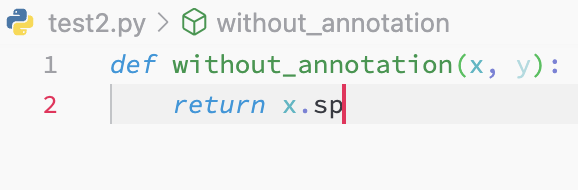
\includegraphics[width=\textwidth]{imgs/without-annotation.png}
                \end{figure}
            \end{block}
        \end{column}
        \begin{column}{0.5\textwidth}
            \begin{block}{With annotation}
                \begin{figure}[h]
                    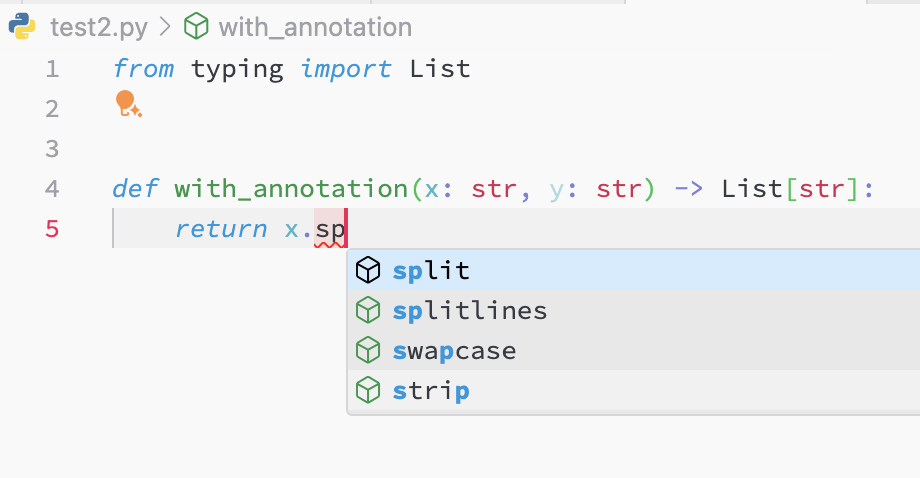
\includegraphics[width=\textwidth]{imgs/with-annotation.png}
                \end{figure}
            \end{block}
        \end{column}
        \end{columns}
        }
        \only<2->{\addtocounter{framenumber}{1}}
        \only<2>{
        Annotation can help us find possibly bugs in the code. For example, if we assign a string to a variable that is supposed to be an integer, the type checker will raise an error.

        \begin{columns}
        \begin{column}{0.5\textwidth}
            \begin{block}{Without annotation}
                \begin{figure}[h]
                    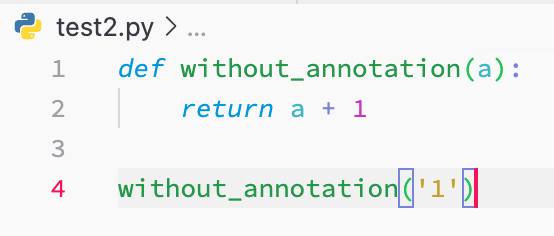
\includegraphics[width=\textwidth]{imgs/without-annotation-2.png}
                \end{figure}
            \end{block}
        \end{column}
        \begin{column}{0.5\textwidth}
            \begin{block}{With annotation}
                \begin{figure}[h]
                    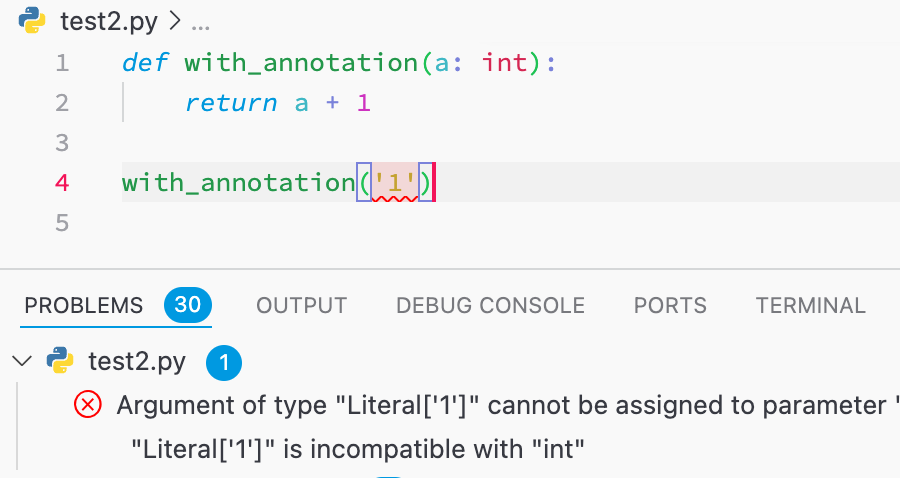
\includegraphics[width=\textwidth]{imgs/with-annotation-2.png}
                \end{figure}
            \end{block}
        \end{column}
        \end{columns}
        }

    \end{frame}
    \begin{frame}[fragile]
        \frametitle{Variable Annotation}

        We can specify the type of a variable by adding a colon and the type after the variable name.

\begin{lstlisting}[language=python]
x: int = 5
y: str = 'Hello, world!'
\end{lstlisting}

        If we can guarantee the correctness of the code, we can ignore type checking using comment {\footnotesize\verb|# type: ignore|} to suppress type checking errors.

        \textbf{Note:} Python is a dynamically typed language, so annotations are not enforced at runtime. Thus, it's not recommended to assign a value of a different type to an annotated variable.
    \end{frame}
    \begin{frame}[fragile]
        \frametitle{Function Annotation}

        We can specify the types of the parameters and return value of a function to improve readability. Function arguments are annotated the same way as variables, while the return value is annotated after an arrow {\footnotesize\verb|->|}.

\begin{lstlisting}[language=python]
def add(x: int, y: int) -> int:
    return x + y

def sum_integers(*args: int) -> int:
    # args is a tuple of integers
    return sum(args)

def sum_integers(**kwargs: int) -> int:
    # kwargs is a dictionary of integers
    return sum(kwargs.values())
\end{lstlisting}

    \end{frame}
    \begin{frame}[fragile]
        \frametitle{Complex Annotations}

        {\footnotesize\verb|typing|} module provides ways to annotate more complex types including container types and union types.

\begin{lstlisting}[language=python]
from __future__ import annotations # Required in Python 3.9- to use `|`
from typing import Any, Dict, List, Optional, Tuple, Union

int_list: List[int] = [1, 2, 3]
int_str_tuple: Tuple[int, str] = (1, 'Hello')
str_int_dict: Dict[str, int] = {'one': 1, 'two': 2}
int_or_str: Union[int, str] = 5
another_int_or_str: int | str = 5
int_or_none: Optional[int] = None
any_type: Any = 5
\end{lstlisting}

        {\footnotesize\itshape\textbf{Remark:} \textbf{(1)} {\scriptsize\verb|Optional[T]|} is equivalent to {\scriptsize\verb|Union[T, None]|}, \textbf{(2)} {\scriptsize\texttt{|}} is only available in Python 3.10+.}
    \end{frame}
    % \section{Scopes}
    % \begin{frame}
    %     \frametitle{Scopes}

    %     Scopes in Python are regions of a program where a namespace is directly accessible. Python has four types of scopes:

    % \end{frame}
    \section{Dive into Standard Libraries}
    \subsection{Math and Random}
    \begin{frame}[fragile]
        \frametitle{Math Functions}

        {\footnotesize\verb|math|} module provides mathematical functions and constants. Functions are restricted to real numbers.

        \begin{itemize}
            \item Square root {\footnotesize\verb|sqrt|} and integer square root {\footnotesize\verb|isqrt|}.
            \item Logarithmic functions {\footnotesize\verb|log|}, {\footnotesize\verb|log2|}, {\footnotesize\verb|log10|}, {\footnotesize\verb|log1p|} and exponentiation functions {\footnotesize\verb|exp|}, {\footnotesize\verb|expm1|}.
            \item Trigonometric functions, hyperbolic functions and their inverses.
            \item Mathematical constants like $\pi$ and $e$.
        \end{itemize}

        {\footnotesize\itshape\textbf{Remark:} Check out \href{https://docs.python.org/3/library/math.html}{\textcolor{darkblue}{official documentation}} for more functions.}
    \end{frame}
    \begin{frame}[fragile]
        \frametitle{Random Numbers}

        {\footnotesize\verb|random|} module provides functions related to randomness.

        \begin{itemize}
            \item Random integers: {\footnotesize\verb|randint|}, {\footnotesize\verb|randrange|}.
            \item Random sequences: {\footnotesize\verb|choice|}, {\footnotesize\verb|choices|}, {\footnotesize\verb|shuffle|}, {\footnotesize\verb|sample|}.
            \item Sample from random distribution: standard uniform {\footnotesize\verb|random|}, uniform {\footnotesize\verb|uniform|}, normal distribution {\footnotesize\verb|gauss|}, exponential distribution {\footnotesize\verb|expovariate|}, etc.
        \end{itemize}

        {\footnotesize\itshape\textbf{Remark:} Check out \href{https://docs.python.org/3/library/random.html}{\textcolor{darkblue}{official documentation}} for more functions.}
    \end{frame}
    \begin{frame}[fragile]
        \frametitle{Example}

        \begin{block}{Example: Integer square roots}
            Randomly generate a series of integers, and calculate their square roots.
        \end{block}

        Key points: random numbers, math functions, loops.

        \pause

\begin{lstlisting}[language=python]
import random
import math

for _ in range(10):
    x = random.randint(1, 100)
    print(f'The square root of {x} is {math.sqrt(x)}.')
\end{lstlisting}
    \end{frame}
    \begin{frame}[fragile]
        \frametitle{Statistics}

        {\footnotesize\verb|statistics|} module provides functions for statistical calculations.

        \begin{itemize}
            \item Measures: {\footnotesize\verb|mean|}, {\footnotesize\verb|median|}, {\footnotesize\verb|mode|}, {\footnotesize\verb|harmonic_mean|}, {\footnotesize\verb|geometric_mean|}.
            \item Variance: {\footnotesize\verb|variance|}, {\footnotesize\verb|pvariance|}, {\footnotesize\verb|stdev|}, {\footnotesize\verb|pstdev|}.
            \item Multi-variates: {\footnotesize\verb|covariance|}, {\footnotesize\verb|correlation|}.
            \item OLS regression: {\footnotesize\verb|linear_regression|}.
        \end{itemize}
        {\footnotesize\itshape\textbf{Remark:} Check out \href{https://docs.python.org/3/library/statistics.html}{\textcolor{darkblue}{official documentation}} for more functions.}
    \end{frame}
    \subsection{OS Interface}
    \begin{frame}[fragile]
        \frametitle{Manipulating Paths}

        {\footnotesize\verb|os.path|} module provides functions for manipulating file paths.

        \begin{itemize}
            \item Combine paths: {\footnotesize\verb|join|}.
            \item Existence: {\footnotesize\verb|exists|}, {\footnotesize\verb|isfile|}, {\footnotesize\verb|isdir|}.
            \item Check file size: {\footnotesize\verb|getsize|}.
            \item Split paths: {\footnotesize\verb|split|}.
            \item List directory: {\footnotesize\verb|listdir|}.
        \end{itemize}

        {\footnotesize\itshape\textbf{Remark:} Check out \href{https://docs.python.org/3/library/os.path.html}{\textcolor{darkblue}{official documentation}} for more functions.}
    \end{frame}
    \begin{frame}[fragile]
        \frametitle{Example}

        \begin{block}{Example: List files in a directory}
            List all files in a directory and print their sizes.
        \end{block}

        Key points: file operations, loops.

        \pause

\begin{lstlisting}[language=python]
import os
for file in os.listdir('.'):
    if os.path.isfile(file):
        size = os.path.getsize(file)
        print(f'{file}: {size} bytes')
\end{lstlisting}
    \end{frame}
    \subsection{Serialization}
    \begin{frame}[fragile]
        \frametitle{JSON Serialization}

        Serialization is the process of converting a Python object into a string or byte stream. Deserialization is the reverse process.

        {\footnotesize\verb|json|} module provides functions for serializing and deserializing JSON objects.

        \begin{itemize}
            \item Serialize: {\footnotesize\verb|dumps|}, {\footnotesize\verb|dump|}.
            \item Deserialize: {\footnotesize\verb|loads|}, {\footnotesize\verb|load|}.
        \end{itemize}

        JSON can only store basic data types including {\footnotesize\verb|None|}, strings, numbers, lists, dictionaries, and booleans. It cannot store complex data types like functions or classes.

        {\footnotesize\itshape\textbf{Remark:} Check out \href{https://docs.python.org/3/library/json.html}{\textcolor{darkblue}{official documentation}} for more functions.}
    \end{frame}
    \begin{frame}[fragile]
        \frametitle{Pickle Serialization}

        {\footnotesize\verb|pickle|} module provides functions for serializing and deserializing Python objects to binary files.

        \begin{itemize}
            \item Serialize: {\footnotesize\verb|dumps|}, {\footnotesize\verb|dump|}.
            \item Deserialize: {\footnotesize\verb|loads|}, {\footnotesize\verb|load|}.
        \end{itemize}

        Pickle can store almost all Python objects, including functions and classes.

        {\footnotesize\itshape\textbf{Remark:} Check out \href{https://docs.python.org/3/library/pickle.html}{\textcolor{darkblue}{official documentation}} for more functions.}
    \end{frame}
    \begin{frame}[fragile]
        \frametitle{Example}

        \begin{block}{Example: Serialize and deserialize a dictionary}
            Serialize a dictionary to a JSON file, then deserialize it back.
        \end{block}

        Key points: serialization, file operations.

        \pause

\begin{lstlisting}[language=python]
import json
with open('data.json', 'w') as f:
    data = {'one': 1, 'two': 2, 'three': 3}
    json.dump(data, f)
with open('data.json', 'r') as f:
    data = json.load(f)
    print(data)
\end{lstlisting}
    \end{frame}
    \section{Iterators}
    \subsection{Comprehension Syntax and Unpacking}
    \begin{frame}[fragile]
        \frametitle{List Comprehension}

        We can embed a for loop inside a list to create a new list. This is called \textbf{list comprehension}.

\begin{lstlisting}[language=python]
# Create a list of squares of numbers from 0 to 9
squares = [x**2 for x in range(10)]
\end{lstlisting}

        List comprehension can also include conditionals.

\begin{lstlisting}[language=python]
# Create a list of even numbers from 0 to 9
evens = [x for x in range(10) if x % 2 == 0]
\end{lstlisting}

    \end{frame}
    \begin{frame}[fragile]
        \frametitle{Other Comprehension}

        Dictionary comprehension and set comprehension are similar to list comprehension.

\begin{lstlisting}[language=python]
# Create a dictionary of squares of numbers from 0 to 9
squares_dict = {x: x**2 for x in range(10)}
squares_set = {x**2 for x in range(10)}
\end{lstlisting}

        Comprehensions are more concise and readable than traditional for loops. They are also faster than for loops. Comprehensions can be nested.

        {\footnotesize\itshape\textbf{Remark:} Check out \href{https://docs.python.org/3/tutorial/datastructures.html#list-comprehensions}{\textcolor{darkblue}{official documentation}} for more information.}
    \end{frame}
    \begin{frame}[fragile]
        \frametitle{Unpacking Iterables}

        We can unpack an iterable into multiple variables.

        \begin{block}{Example}
            {\footnotesize\verb|x, y = (1, 2)|} assigns 1 to {\footnotesize\verb|x|} and 2 to {\footnotesize\verb|y|}.
        \end{block}

        When the number of variables is less than the number of elements in the iterable, we can use an asterisk {\footnotesize\verb|*|} to collect the remaining elements into a list.

        \begin{block}{Example}
            {\footnotesize\verb|x, *y = (1, 2, 3)|} assigns 1 to {\footnotesize\verb|x|} and {\footnotesize\verb|[2, 3]|} to {\footnotesize\verb|y|}.
        \end{block}
    \end{frame}
    \begin{frame}[fragile]
        \frametitle{Example}

        \begin{block}{Example: Unpacking}
            Swap the values of two variables {\footnotesize\verb|x|} and {\footnotesize\verb|y|}.
        \end{block}

        Key points: variables, unpacking.

        \pause

\begin{lstlisting}[language=python]
x, y = 1, 2
x, y = y, x
print(x, y)
\end{lstlisting}

    \end{frame}
    \begin{frame}[fragile]
        \frametitle{Another Unpacking}

        When defining lists and sets, we can use the asterisk {\footnotesize\verb|*|} to unpack another iterable.

        \begin{block}{Example}
            {\footnotesize\verb|[1, 2, *range(3, 6)]|} is equivalent to {\footnotesize\verb|[1, 2, 3, 4, 5]|}.
        \end{block}

        When defining dictionaries, we can use the double asterisk {\footnotesize\verb|**|} to unpack another dictionary.

        \begin{block}{Example}
            {\footnotesize\verb|{'one': 1, **{'two': 2, 'three': 3}}|} is equivalent to {\footnotesize\verb|{'one': 1, 'two': 2, 'three': 3}|}.
        \end{block}
    \end{frame}
    \subsection{Rethink For-Loops}
    \begin{frame}[fragile]
        \frametitle{Rethink For-Loops}

        Syntax of {\footnotesize\verb|for|} loops:

\begin{lstlisting}[language=python]
for item in sequence:
    # Do something with item
\end{lstlisting}

        {\footnotesize\verb|for|} loop takes an item from the sequence and then perform some action on it, which is more specifically called \textbf{iteration}. An \textbf{iterable} is an object that supports iterating (i.e., it can be used in a {\footnotesize\verb|for|} loop). Any container type like lists, tuples, dictionaries, sets, strings, and files are iterables.

    \end{frame}
    \begin{frame}[fragile]
        \frametitle{Iterators}

        An \textbf{iterator} can be considered as a stream of objects or a ``lazy'' iterable, which generates elements on the fly. Since it does not store all elements in memory, it is more memory efficient than a container.

        We can use the {\footnotesize\verb|for|} loop to iterate over an iterator, or use the {\footnotesize\verb|next|} function to fetch the next element. However, iterators can only be iterated once (i.e. it cannot go back). After the iterator is exhausted, it cannot be reused. We need to create a new iterator to iterate again.

        Use {\footnotesize\verb|iter|} function to convert an iterable to an iterator. Iterators are also iterables so they also support unpacking.

        {\footnotesize\itshape\textbf{Remark:} \textbf{(1)} An iterator can ``contain'' infinite elements. \textbf{(2)} When an iterator is exhausted, calling {\scriptsize\verb|next|} will raise a {\scriptsize\verb|StopIteration|} exception. \textbf{(3)} do not unpack an iterator with infinite elements.}
    \end{frame}
    \subsection{Generators}
    \begin{frame}[fragile]
        \frametitle{Generator Syntax}

        We can easily use the {\footnotesize\verb|yield|} keyword to turn a function into a iterator. When the function is called, an iterator (namely a generator) instead of the return value is returned.

\begin{lstlisting}[language=python]
def count(n):
    for i in range(n):
        yield i
\end{lstlisting}

        This function turns an integer $n$ into a generator that generates numbers from 0 to $n-1$.
    \end{frame}
    \begin{frame}[fragile]
        \frametitle{Execution Flow of Generators}

        Generators break the normal workflow of functions. Calling {\footnotesize\verb|next|} function on a generator will execute the function until the next {\footnotesize\verb|yield|} statement and return the value. The generator will pause at the {\footnotesize\verb|yield|} statement until the next call to {\footnotesize\verb|next|}.

        Reaching the end of the function or executing a {\footnotesize\verb|return|} statement will raise a {\footnotesize\verb|StopIteration|} exception.
    \end{frame}
    \begin{frame}[fragile]
        \frametitle{Generator Expressions}

        Another way to create generators is to use generator expressions. Generator expressions are similar to list comprehensions, but use parentheses instead of square brackets.

        \begin{block}{Example}
            {\footnotesize\verb|(x**2 for x in range(10))|} is a generator expression that generates squares of numbers from 0 to 9.
        \end{block}

        {\footnotesize\itshape\textbf{Remark:} Notices that generators are not sequences, so they cannot be indexed.}
    \end{frame}
    \begin{frame}[fragile]
        \frametitle{Example}

        \begin{block}{Example: Fibonacci sequence}
            Create a generator that generates the Fibonacci sequence.
        \end{block}

        Key points: generators, infinite iterators.

        \pause

\begin{lstlisting}[language=python]
def fibonacci():
    a, b = 0, 1
    while True:
        yield a
        a, b = b, a + b

fib = fibonacci()
for _ in range(10):
    print(next(fib))
\end{lstlisting}
    \end{frame}
    \subsection{Iterator Utilities}
    \begin{frame}[fragile]
        \frametitle{{\normalsize\texttt{itertools}} Module}

        {\footnotesize\verb|itertools|} module provides functions for creating iterators for common tasks.

        \begin{itemize}
            \item Producing infinite iterators: {\footnotesize\verb|count|}, {\footnotesize\verb|cycle|}, {\footnotesize\verb|repeat|}.
            \item Chaining iterators: {\footnotesize\verb|chain|}.
            \item Combining iterators: {\footnotesize\verb|product|}, {\footnotesize\verb|permutations|}, {\footnotesize\verb|combinations|}.
            \item Breakdown iterators: {\footnotesize\verb|tee|}, {\footnotesize\verb|pairwise|}.
        \end{itemize}
    \end{frame}
    \begin{frame}[fragile]
        \frametitle{Built-in Functions}

        Python provides several built-in functions that work with iterators.

        \begin{itemize}
            \item {\footnotesize\verb|all|}, {\footnotesize\verb|any|}: Check if all or any elements in an iterator are true.
            \item {\footnotesize\verb|enumerate|}: Iterate over an iterator and yield the index and element.
            \item {\footnotesize\verb|zip|}: Combine elements from multiple iterators into an iterator of tuples.
            \item High-order functions including {\footnotesize\verb|filter|}, {\footnotesize\verb|map|} will be be covered later.
        \end{itemize}
    \end{frame}
    \begin{frame}[fragile]
        \frametitle{Example}

        \begin{block}{Example: List to dictionary}
            Convert two lists {\footnotesize\verb|['one', 'two', 'three']|} and {\footnotesize\verb|[1, 2, 3]|} into a dictionary.
        \end{block}

        Key points: iterators, built-in functions, dictionary comprehension.

        \pause

\begin{lstlisting}[language=python]
keys = ['one', 'two', 'three']
values = [1, 2, 3]
data = {k: v for k, v in zip(keys, values)}
print(data)
\end{lstlisting}

    \end{frame}
    \section{Introduction to Functional Programming}
    \subsection{Callables and Lambda Functions}
    \begin{frame}[fragile]
        \frametitle{Callables}

        In Python, functions are first-class objects, which means they share the same properties as other objects like integers or strings. Functions can be assigned to variables, passed as arguments, and returned from other functions. If an object can be called (like we call a function), it is called a \textbf{callable}.

\begin{lstlisting}[language=python]
def get_print():
    return print # Return the built-in print function

print_func = get_print() # Assign the print function to a variable
print_func('Hello, world!')
\end{lstlisting}

        {\footnotesize\itshape\textbf{Remark:} Variable scope issues may arise when using functions as return values.}

    \end{frame}
    \begin{frame}[fragile]
        \frametitle{Lambda Functions}

        For some simple functions, we can use lambda functions to define them in a more concise way.

        \begin{block}{Lambda function syntax}
            {\footnotesize\verb|lambda arguments: expression|}
        \end{block}

\begin{lstlisting}[language=python]
add = lambda x, y: x + y
print(add(1, 2)) # Output: 3
\end{lstlisting}

        {\footnotesize\itshape\textbf{Remark:} Lambda functions can only contain a single expression.}
    \end{frame}
    \subsection{Higher-Order Functions}
    \begin{frame}[fragile]
        \frametitle{Higher-Order Functions}

        Functions that take other functions as arguments or return functions are called \textbf{higher-order functions}. {\footnotesize\verb|map|} and {\footnotesize\verb|filter|} are two common higher-order functions.

        \begin{itemize}
            \item {\footnotesize\verb|map|}: Apply a function to each element in an iterator.
            \item {\footnotesize\verb|filter|}: Filter elements in an iterator based on a function. Elements are passed to the function, and only those that return {\footnotesize\verb|True|} are kept.
        \end{itemize}

        {\footnotesize\verb|functools|} module provides more higher-order functions like {\footnotesize\verb|reduce|} and {\footnotesize\verb|partial|}.

        {\footnotesize\itshape\textbf{Remark:} {\scriptsize\verb|map|} and {\scriptsize\verb|filter|} are lazy, the function is only called when the iterator is iterated.}
    \end{frame}
    \begin{frame}[fragile]
        \frametitle{Example}

        \begin{block}{Example: Squares of even numbers}
            Given a list of numbers, filter out the even numbers and calculate their squares.
        \end{block}

        \pause

\begin{lstlisting}[language=python]
numbers = [1, 2, 3, 4, 5, 6, 7, 8, 9, 10]
squares = map(lambda x: x**2, filter(lambda x: x % 2 == 0, numbers))
print([*squares])
\end{lstlisting}
    \end{frame}
    \section{Further Reading}
    \begin{frame}[fragile]
        \frametitle{``Battery Included''}

        Python is known for its ``batteries included'' philosophy, which means that the standard library provides a wide range of modules for common tasks. Apart from the modules mentioned in this lecture, there are many other modules in the standard library that can help you with various tasks.

        \begin{itemize}
            \item {\footnotesize\verb|re|}: Regular expressions.
            \item {\footnotesize\verb|datetime|} and {\footnotesize\verb|time|}: Date and time manipulation.
            \item {\footnotesize\verb|heapq|} and {\footnotesize\verb|bisect|}: Heap queues and bisect algorithms.
            \item {\footnotesize\verb|collections|}, {\footnotesize\verb|dataclasses|}: Additional data structures.
            \item {\footnotesize\verb|sqlite3|}: SQLite database interface.
            \item {\footnotesize\verb|subprocess|}: Calling external commands.
        \end{itemize}
    \end{frame}
    \begin{frame}
        \frametitle{Dive Deeper}

        Other advanced topics in Python programming include:

        \begin{itemize}
            \item Asynchronous programming
            \item Functional programming
            \item Object-oriented programming
        \end{itemize}

        The following books are recommended for further reading:

        \begin{itemize}
            \item \textit{Fluent Python} by Luciano Ramalho
            \item \textit{Python Cookbook} by David Beazley and Brian K. Jones
        \end{itemize}
    \end{frame}
    \begin{frame}
        \mythanks
    \end{frame}
\end{document}